\newpage
\subsection{Declaring classes and attributes}
\visHeader
\hypertarget{static:classes vis}{}

\begin{itemize}

\item[$\blacktriangleright$] Double-click your \texttt{LearningBoxLanguage} diagram to ensure it's open.

\vspace{0.5cm}

\item[$\blacktriangleright$] To the left of the workbench in EA, a \emph{Toolbox} containing the types available in Ecore for metamodelling should have
appeared\footnote{If not, choose ``Diagram/Diagram Toolbox'' to show the current toolbox.} (Fig.~\ref{fig:eclass}). Click on \texttt{EClass}, then click again
in the open diagram.

\vspace{0.5cm}

\begin{figure}[htbp]
	\centering
  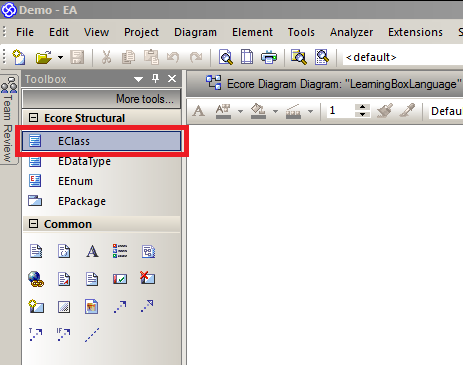
\includegraphics[width=0.7\textwidth]{ea_createEClass}
	\caption{Create an EClass}
	\label{fig:eclass}
\end{figure}

\vspace{0.5cm}

\item[$\blacktriangleright$] In the dialogue that pops-up, enter `Box' as the name of the class and click \texttt{OK} (Fig.~\ref{fig:eclass_properties}).
This dialogue can always be invoked again by double-clicking the class, and contains many other properties we'll investigate later in the handbook.
In general, a similar ``properties'' dialogues can be opened in the same fashion for almost every element in EA.

\begin{figure}[ht]
	\centering
  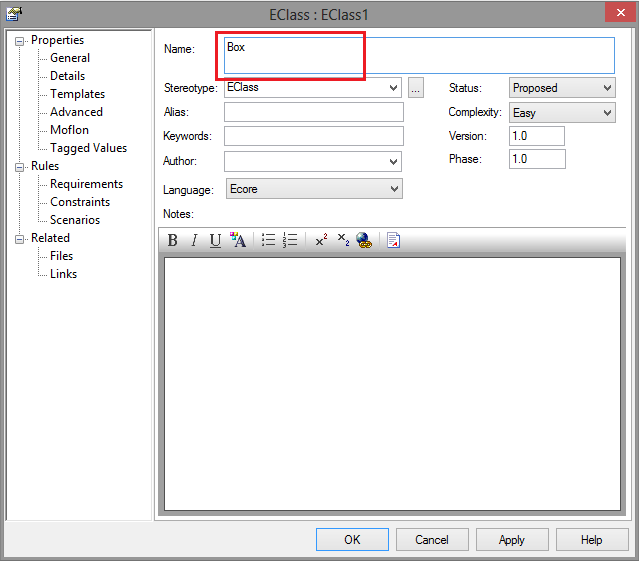
\includegraphics[width=0.8\textwidth]{ea_propertiesEClass}
	\caption{Edit properties of an EClass}
	\label{fig:eclass_properties}
\end{figure}

\newpage

\item[$\blacktriangleright$] After creating \texttt{Box}, your EA workspace should resemble Fig.~\ref{fig:eclass_completed}.

\begin{figure}[htbp]
	\centering
  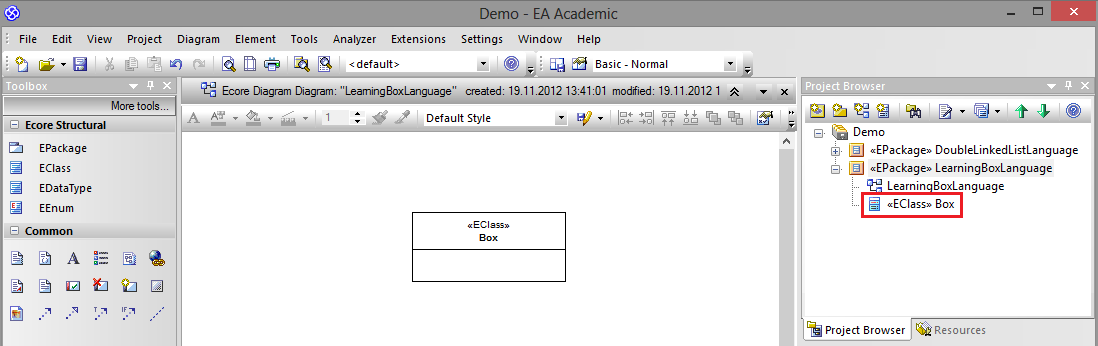
\includegraphics[width=1\textwidth]{ea_afterBoxCreation}
	\caption{State after creating \texttt{Box}}
	\label{fig:eclass_completed}
\end{figure}

\item[$\blacktriangleright$] Now create \texttt{Partition} and \texttt{Card} the same way, until your workspace resembles Fig.~\ref{fig:all_eclasses}.
These are the main models for our learning box.

\vspace{0.5cm}

\item[$\blacktriangleright$] Now choose \texttt{Box}, right-click to call up the context menu, and choose ``Features \& Properties/Attributes..''
(Fig.~\ref{fig:attribute}).

\begin{figure}[htbp]
	\centering
  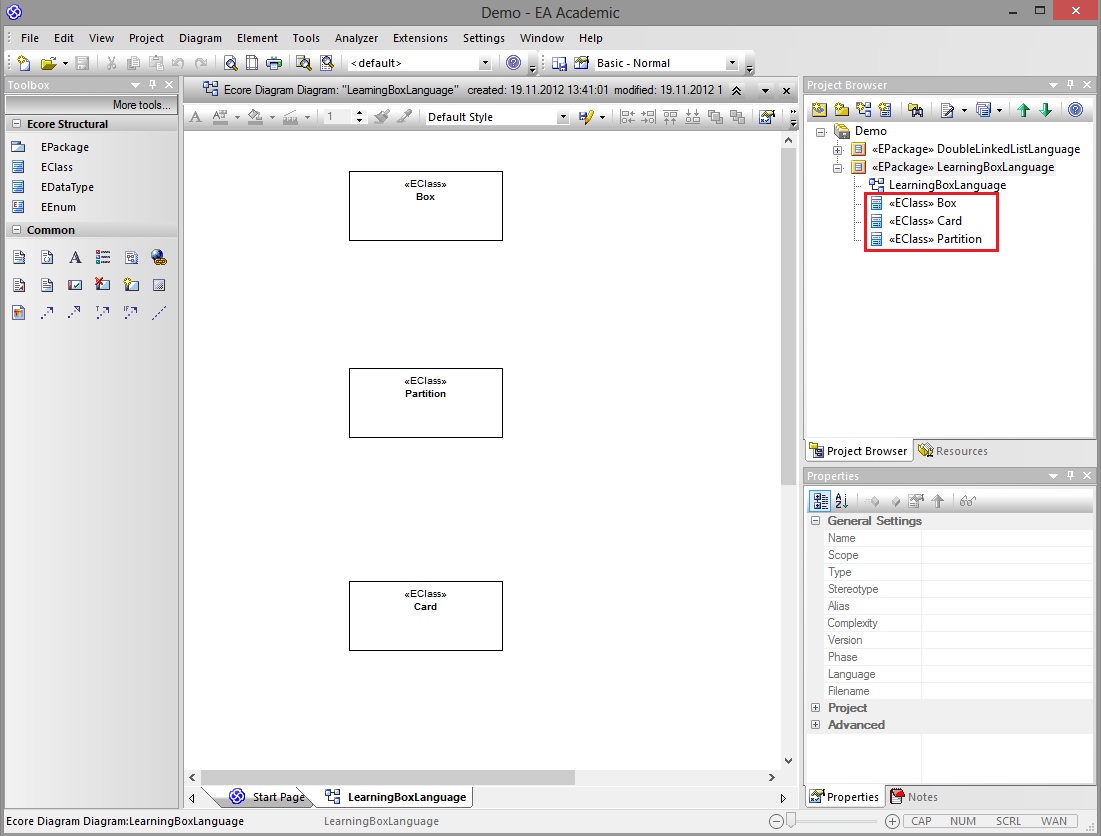
\includegraphics[width=0.9\textwidth]{ea_createPartitionCard}
	\caption{All classes for the metamodel}
	\label{fig:all_eclasses}
\end{figure}

\begin{figure}[htbp]
	\centering
  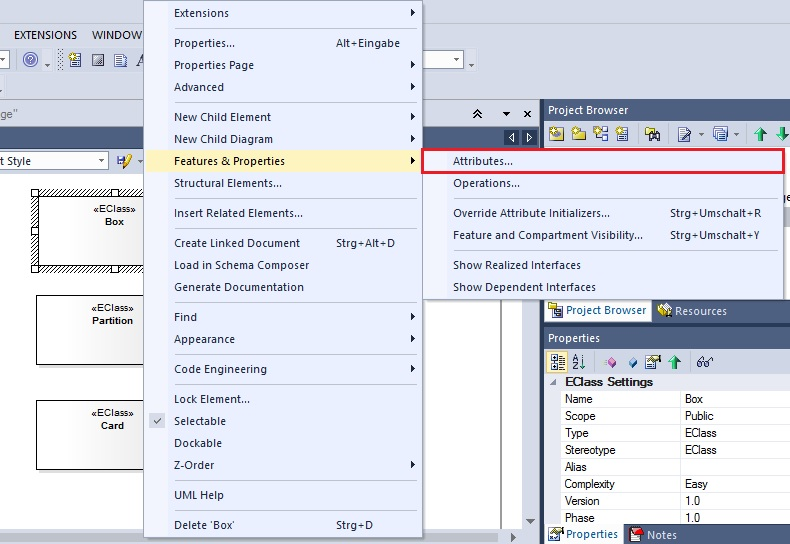
\includegraphics[width=0.7\textwidth]{ea_contextAddAttribute}
	\caption{Context menu for an EClass}
	\label{fig:attribute}
\end{figure}
\FloatBarrier

\item[$\blacktriangleright$] In the dialogue that pops-up, enter `name' as the name of the attribute, choose \texttt{EString} as its type, and press
\texttt{Save} (Fig.~\ref{fig:attribute_properties}). New attributes for the same class can be added by choosing \texttt{New}.

\begin{figure}[htbp]
	\centering
  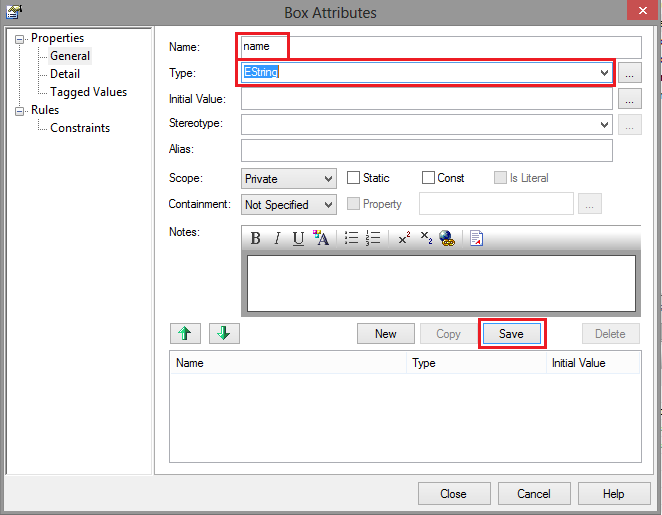
\includegraphics[width=0.6\textwidth]{ea_addingAttributes}
	\caption{Adding attributes to an EClass}
	\label{fig:attribute_properties}
\end{figure}

\item[$\blacktriangleright$] Add attributes to all classes until your workspace resembles Fig.~\ref{fig:attribute_completed}.

\begin{figure}[htbp]
	\centering
  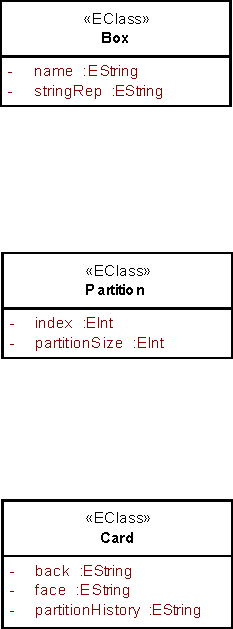
\includegraphics[width=0.23\textwidth]{ea_allAttributes}
	\caption{Main classes with attributes}
	\label{fig:attribute_completed}
\end{figure}
\FloatBarrier

\item[$\blacktriangleright$] Closing message.

\fancyfoot[R]{$\triangleright$ \hyperlink{static:references splash}{Next}}

\end{itemize}
